
%% bare_conf.tex
%% V1.3
%% 2007/01/11
%% by Michael Shell
%% See:
%% http://www.michaelshell.org/
%% for current contact information.
%%
%% This is a skeleton file demonstrating the use of IEEEtran.cls
%% (requires IEEEtran.cls version 1.7 or later) with an IEEE conference paper.
%%
%% Support sites:
%% http://www.michaelshell.org/tex/ieeetran/
%% http://www.ctan.org/tex-archive/macros/latex/contrib/IEEEtran/
%% and
%% http://www.ieee.org/

%%*************************************************************************
%% Legal Notice:
%% This code is offered as-is without any warranty either expressed or
%% implied; without even the implied warranty of MERCHANTABILITY or
%% FITNESS FOR A PARTICULAR PURPOSE! 
%% User assumes all risk.
%% In no event shall IEEE or any contributor to this code be liable for
%% any damages or losses, including, but not limited to, incidental,
%% consequential, or any other damages, resulting from the use or misuse
%% of any information contained here.
%%
%% All comments are the opinions of their respective authors and are not
%% necessarily endorsed by the IEEE.
%%
%% This work is distributed under the LaTeX Project Public License (LPPL)
%% ( http://www.latex-project.org/ ) version 1.3, and may be freely used,
%% distributed and modified. A copy of the LPPL, version 1.3, is included
%% in the base LaTeX documentation of all distributions of LaTeX released
%% 2003/12/01 or later.
%% Retain all contribution notices and credits.
%% ** Modified files should be clearly indicated as such, including  **
%% ** renaming them and changing author support contact information. **
%%
%% File list of work: IEEEtran.cls, IEEEtran_HOWTO.pdf, bare_adv.tex,
%%                    bare_conf.tex, bare_jrnl.tex, bare_jrnl_compsoc.tex
%%*************************************************************************

% *** Authors should verify (and, if needed, correct) their LaTeX system  ***
% *** with the testflow diagnostic prior to trusting their LaTeX platform ***
% *** with production work. IEEE's font choices can trigger bugs that do  ***
% *** not appear when using other class files.                            ***
% The testflow support page is at:
% http://www.michaelshell.org/tex/testflow/



% Note that the a4paper option is mainly intended so that authors in
% countries using A4 can easily print to A4 and see how their papers will
% look in print - the typesetting of the document will not typically be
% affected with changes in paper size (but the bottom and side margins will).
% Use the testflow package mentioned above to verify correct handling of
% both paper sizes by the user's LaTeX system.
%
% Also note that the "draftcls" or "draftclsnofoot", not "draft", option
% should be used if it is desired that the figures are to be displayed in
% draft mode.
%
\documentclass[conference]{IEEEtran}
% Add the compsoc option for Computer Society conferences.
%
% If IEEEtran.cls has not been installed into the LaTeX system files,
% manually specify the path to it like:
% \documentclass[conference]{../sty/IEEEtran}





% Some very useful LaTeX packages include:
% (uncomment the ones you want to load)


% *** MISC UTILITY PACKAGES ***
%
%\usepackage{ifpdf}
% Heiko Oberdiek's ifpdf.sty is very useful if you need conditional
% compilation based on whether the output is pdf or dvi.
% usage:
% \ifpdf
%   % pdf code
% \else
%   % dvi code
% \fi
% The latest version of ifpdf.sty can be obtained from:
% http://www.ctan.org/tex-archive/macros/latex/contrib/oberdiek/
% Also, note that IEEEtran.cls V1.7 and later provides a builtin
% \ifCLASSINFOpdf conditional that works the same way.
% When switching from latex to pdflatex and vice-versa, the compiler may
% have to be run twice to clear warning/error messages.






% *** CITATION PACKAGES ***
%
%\usepackage{cite}
% cite.sty was written by Donald Arseneau
% V1.6 and later of IEEEtran pre-defines the format of the cite.sty package
% \cite{} output to follow that of IEEE. Loading the cite package will
% result in citation numbers being automatically sorted and properly
% "compressed/ranged". e.g., [1], [9], [2], [7], [5], [6] without using
% cite.sty will become [1], [2], [5]--[7], [9] using cite.sty. cite.sty's
% \cite will automatically add leading space, if needed. Use cite.sty's
% noadjust option (cite.sty V3.8 and later) if you want to turn this off.
% cite.sty is already installed on most LaTeX systems. Be sure and use
% version 4.0 (2003-05-27) and later if using hyperref.sty. cite.sty does
% not currently provide for hyperlinked citations.
% The latest version can be obtained at:
% http://www.ctan.org/tex-archive/macros/latex/contrib/cite/
% The documentation is contained in the cite.sty file itself.


\usepackage{enumerate}
\usepackage{rotating}
\usepackage{url}

% *** GRAPHICS RELATED PACKAGES ***
%
\ifCLASSINFOpdf
  % \usepackage[pdftex]{graphicx}
  % declare the path(s) where your graphic files are
  % \graphicspath{{../pdf/}{../jpeg/}}
  % and their extensions so you won't have to specify these with
  % every instance of \includegraphics
  % \DeclareGraphicsExtensions{.pdf,.jpeg,.png}
\else
  % or other class option (dvipsone, dvipdf, if not using dvips). graphicx
  % will default to the driver specified in the system graphics.cfg if no
  % driver is specified.
  % \usepackage[dvips]{graphicx}
  % declare the path(s) where your graphic files are
  % \graphicspath{{../eps/}}
  % and their extensions so you won't have to specify these with
  % every instance of \includegraphics
  % \DeclareGraphicsExtensions{.eps}
\fi
% graphicx was written by David Carlisle and Sebastian Rahtz. It is
% required if you want graphics, photos, etc. graphicx.sty is already
% installed on most LaTeX systems. The latest version and documentation can
% be obtained at: 
% http://www.ctan.org/tex-archive/macros/latex/required/graphics/
% Another good source of documentation is "Using Imported Graphics in
% LaTeX2e" by Keith Reckdahl which can be found as epslatex.ps or
% epslatex.pdf at: http://www.ctan.org/tex-archive/info/
%
% latex, and pdflatex in dvi mode, support graphics in encapsulated
% postscript (.eps) format. pdflatex in pdf mode supports graphics
% in .pdf, .jpeg, .png and .mps (metapost) formats. Users should ensure
% that all non-photo figures use a vector format (.eps, .pdf, .mps) and
% not a bitmapped formats (.jpeg, .png). IEEE frowns on bitmapped formats
% which can result in "jaggedy"/blurry rendering of lines and letters as
% well as large increases in file sizes.
%
% You can find documentation about the pdfTeX application at:
% http://www.tug.org/applications/pdftex





% *** MATH PACKAGES ***
%
%\usepackage[cmex10]{amsmath}
% A popular package from the American Mathematical Society that provides
% many useful and powerful commands for dealing with mathematics. If using
% it, be sure to load this package with the cmex10 option to ensure that
% only type 1 fonts will utilized at all point sizes. Without this option,
% it is possible that some math symbols, particularly those within
% footnotes, will be rendered in bitmap form which will result in a
% document that can not be IEEE Xplore compliant!
%
% Also, note that the amsmath package sets \interdisplaylinepenalty to 10000
% thus preventing page breaks from occurring within multiline equations. Use:
%\interdisplaylinepenalty=2500
% after loading amsmath to restore such page breaks as IEEEtran.cls normally
% does. amsmath.sty is already installed on most LaTeX systems. The latest
% version and documentation can be obtained at:
% http://www.ctan.org/tex-archive/macros/latex/required/amslatex/math/





% *** SPECIALIZED LIST PACKAGES ***
%
%\usepackage{algorithmic}
% algorithmic.sty was written by Peter Williams and Rogerio Brito.
% This package provides an algorithmic environment fo describing algorithms.
% You can use the algorithmic environment in-text or within a figure
% environment to provide for a floating algorithm. Do NOT use the algorithm
% floating environment provided by algorithm.sty (by the same authors) or
% algorithm2e.sty (by Christophe Fiorio) as IEEE does not use dedicated
% algorithm float types and packages that provide these will not provide
% correct IEEE style captions. The latest version and documentation of
% algorithmic.sty can be obtained at:
% http://www.ctan.org/tex-archive/macros/latex/contrib/algorithms/
% There is also a support site at:
% http://algorithms.berlios.de/index.html
% Also of interest may be the (relatively newer and more customizable)
% algorithmicx.sty package by Szasz Janos:
% http://www.ctan.org/tex-archive/macros/latex/contrib/algorithmicx/




% *** ALIGNMENT PACKAGES ***
%
%\usepackage{array}
% Frank Mittelbach's and David Carlisle's array.sty patches and improves
% the standard LaTeX2e array and tabular environments to provide better
% appearance and additional user controls. As the default LaTeX2e table
% generation code is lacking to the point of almost being broken with
% respect to the quality of the end results, all users are strongly
% advised to use an enhanced (at the very least that provided by array.sty)
% set of table tools. array.sty is already installed on most systems. The
% latest version and documentation can be obtained at:
% http://www.ctan.org/tex-archive/macros/latex/required/tools/


%\usepackage{mdwmath}
%\usepackage{mdwtab}
% Also highly recommended is Mark Wooding's extremely powerful MDW tools,
% especially mdwmath.sty and mdwtab.sty which are used to format equations
% and tables, respectively. The MDWtools set is already installed on most
% LaTeX systems. The lastest version and documentation is available at:
% http://www.ctan.org/tex-archive/macros/latex/contrib/mdwtools/


% IEEEtran contains the IEEEeqnarray family of commands that can be used to
% generate multiline equations as well as matrices, tables, etc., of high
% quality.


%\usepackage{eqparbox}
% Also of notable interest is Scott Pakin's eqparbox package for creating
% (automatically sized) equal width boxes - aka "natural width parboxes".
% Available at:
% http://www.ctan.org/tex-archive/macros/latex/contrib/eqparbox/





% *** SUBFIGURE PACKAGES ***
%\usepackage[tight,footnotesize]{subfigure}
% subfigure.sty was written by Steven Douglas Cochran. This package makes it
% easy to put subfigures in your figures. e.g., "Figure 1a and 1b". For IEEE
% work, it is a good idea to load it with the tight package option to reduce
% the amount of white space around the subfigures. subfigure.sty is already
% installed on most LaTeX systems. The latest version and documentation can
% be obtained at:
% http://www.ctan.org/tex-archive/obsolete/macros/latex/contrib/subfigure/
% subfigure.sty has been superceeded by subfig.sty.



%\usepackage[caption=false]{caption}
%\usepackage[font=footnotesize]{subfig}
% subfig.sty, also written by Steven Douglas Cochran, is the modern
% replacement for subfigure.sty. However, subfig.sty requires and
% automatically loads Axel Sommerfeldt's caption.sty which will override
% IEEEtran.cls handling of captions and this will result in nonIEEE style
% figure/table captions. To prevent this problem, be sure and preload
% caption.sty with its "caption=false" package option. This is will preserve
% IEEEtran.cls handing of captions. Version 1.3 (2005/06/28) and later 
% (recommended due to many improvements over 1.2) of subfig.sty supports
% the caption=false option directly:
%\usepackage[caption=false,font=footnotesize]{subfig}
%
% The latest version and documentation can be obtained at:
% http://www.ctan.org/tex-archive/macros/latex/contrib/subfig/
% The latest version and documentation of caption.sty can be obtained at:
% http://www.ctan.org/tex-archive/macros/latex/contrib/caption/




% *** FLOAT PACKAGES ***
%
%\usepackage{fixltx2e}
% fixltx2e, the successor to the earlier fix2col.sty, was written by
% Frank Mittelbach and David Carlisle. This package corrects a few problems
% in the LaTeX2e kernel, the most notable of which is that in current
% LaTeX2e releases, the ordering of single and double column floats is not
% guaranteed to be preserved. Thus, an unpatched LaTeX2e can allow a
% single column figure to be placed prior to an earlier double column
% figure. The latest version and documentation can be found at:
% http://www.ctan.org/tex-archive/macros/latex/base/



%\usepackage{stfloats}
% stfloats.sty was written by Sigitas Tolusis. This package gives LaTeX2e
% the ability to do double column floats at the bottom of the page as well
% as the top. (e.g., "\begin{figure*}[!b]" is not normally possible in
% LaTeX2e). It also provides a command:
%\fnbelowfloat
% to enable the placement of footnotes below bottom floats (the standard
% LaTeX2e kernel puts them above bottom floats). This is an invasive package
% which rewrites many portions of the LaTeX2e float routines. It may not work
% with other packages that modify the LaTeX2e float routines. The latest
% version and documentation can be obtained at:
% http://www.ctan.org/tex-archive/macros/latex/contrib/sttools/
% Documentation is contained in the stfloats.sty comments as well as in the
% presfull.pdf file. Do not use the stfloats baselinefloat ability as IEEE
% does not allow \baselineskip to stretch. Authors submitting work to the
% IEEE should note that IEEE rarely uses double column equations and
% that authors should try to avoid such use. Do not be tempted to use the
% cuted.sty or midfloat.sty packages (also by Sigitas Tolusis) as IEEE does
% not format its papers in such ways.





% *** PDF, URL AND HYPERLINK PACKAGES ***
%
%\usepackage{url}
% url.sty was written by Donald Arseneau. It provides better support for
% handling and breaking URLs. url.sty is already installed on most LaTeX
% systems. The latest version can be obtained at:
% http://www.ctan.org/tex-archive/macros/latex/contrib/misc/
% Read the url.sty source comments for usage information. Basically,
% \url{my_url_here}.





% *** Do not adjust lengths that control margins, column widths, etc. ***
% *** Do not use packages that alter fonts (such as pslatex).         ***
% There should be no need to do such things with IEEEtran.cls V1.6 and later.
% (Unless specifically asked to do so by the journal or conference you plan
% to submit to, of course. )


% correct bad hyphenation here
\hyphenation{op-tical net-works semi-conduc-tor}


\begin{document}
%
% paper title
% can use linebreaks \\ within to get better formatting as desired
\title{Active Code Completion}


% author names and affiliations
% use a multiple column layout for up to three different
% affiliations
\author{\IEEEauthorblockN{Cyrus Omar, YoungSeok Yoon, Thomas D. LaToza, Brad A. Myers}
\IEEEauthorblockA{School of Computer Science\\
Carnegie Mellon University\\
Pittsburgh, PA, USA\\
\{comar,youngseok,tlatoza,bam\}@cs.cmu.edu}
\texttt{\url{https://github.com/cyrus-/graphite}}
}

% conference papers do not typically use \thanks and this command
% is locked out in conference mode. If really needed, such as for
% the acknowledgment of grants, issue a \IEEEoverridecommandlockouts
% after \documentclass

% for over three affiliations, or if they all won't fit within the width
% of the page, use this alternative format:
% 
%\author{\IEEEauthorblockN{Michael Shell\IEEEauthorrefmark{1},
%Homer Simpson\IEEEauthorrefmark{2},
%James Kirk\IEEEauthorrefmark{3}, 
%Montgomery Scott\IEEEauthorrefmark{3} and
%Eldon Tyrell\IEEEauthorrefmark{4}}
%\IEEEauthorblockA{\IEEEauthorrefmark{1}School of Electrical and Computer Engineering\\
%Georgia Institute of Technology,
%Atlanta, Georgia 30332--0250\\ Email: see http://www.michaelshell.org/contact.html}
%\IEEEauthorblockA{\IEEEauthorrefmark{2}Twentieth Century Fox, Springfield, USA\\
%Email: homer@thesimpsons.com}
%\IEEEauthorblockA{\IEEEauthorrefmark{3}Starfleet Academy, San Francisco, California 96678-2391\\
%Telephone: (800) 555--1212, Fax: (888) 555--1212}
%\IEEEauthorblockA{\IEEEauthorrefmark{4}Tyrell Inc., 123 Replicant Street, Los Angeles, California 90210--4321}}




% use for special paper notices
%\IEEEspecialpapernotice{(Invited Paper)}




% make the title area
% \maketitle


% IEEEtran.cls defaults to using nonbold math in the Abstract.
% This preserves the distinction between vectors and scalars. However,
% if the conference you are submitting to favors bold math in the abstract,
% then you can use LaTeX's standard command \boldmath at the very start
% of the abstract to achieve this. Many IEEE journals/conferences frown on
% math in the abstract anyway.

% no keywords




% For peer review papers, you can put extra information on the cover
% page as needed:
% \ifCLASSOPTIONpeerreview
% \begin{center} \bfseries EDICS Category: 3-BBND \end{center}
% \fi
%
% For peerreview papers, this IEEEtran command inserts a page break and
% creates the second title. It will be ignored for other modes.
% \IEEEpeerreviewmaketitle



\section{Developer Survey}

Prior to implementation, we conducted a large online survey of professional software developers in order to extract criteria that govern whether our system would be useful to them. More specifically, we sought to address the following questions:

\begin{itemize}
\item What are specific use cases for active code completion in a professional setting? 
\item What are some functional criteria that predict whether a class would benefit from active code completion?
\item What are some usability criteria that should govern palette interface designs?
\item Which capabilities must a active code completion architecture support to enable these use cases and designs?
\end{itemize}

% In order to convey the active code completion concept clearly, we came up with three different use cases where we belive the active code completion technique will benefit developers frequently. For each use case, we designed three mock-up screenshots and showed them in sequence: before invoking the palette, during the interaction with the palette, and after the palette is closed and code is generated. By doing this, the respondents could understand the concept precisely and give useful feedback relevant to the above questions.

We posted a link to our survey on a popular  collaborative filtering website \cite{mehta_robust_2007} called {\tt /r/programming} on reddit.com\footnote{\texttt{http://www.reddit.com/r/programming}}. At the time of our study, the website listed approximately 340,000, though members were not required to registered to read the content,  and contained content that could be considered relevant to our intended audience. An additional 22 participants were recruited using a mass email to local computer science graduate students. The recruitment materials in both cases stated that we were seeking developers ``familiar with an object-oriented programming language like Java, C\# or Visual Basic and an integrated development environment like Eclipse or Visual Studio''.

Participants were asked to take an online survey that would take approximately 20 minutes to complete. Of the 696 people who started the survey by answering the first question, 473 participants completed it. Of these, 16 participants were computer science graduate students at Carnegie Mellon and 457 were from \texttt{/r/programming}.

Their responses revealed a number of interesting use cases and non-trivial design constraints for active code completion systems. Many of these findings can also be generalized to constrain the design of visual programming languages, particularly those that aim be useful to professional developers, rather than novice programmers (e.g., Barista \cite{ko_barista:_2006}). We summarize the survey questions and the results in the following subsections.
% In fact, active code completion can be considered a hybrid approach that borrows interaction techniques from visual languages while remaining compatible with conventional representations of program logic. This may help address some of the usability challenges previously associated with visual languages (cf. [?]).

\subsection{Familiarity with Programming Languages and Editors}

We first asked their level of familiarity with several programming languages, on a five-point Likert scale ranging from ``None'' to ``Expert''. 61.1\% of the respondents expressed themselves as experts on at least one language, and 35.7\% were very familiar with at least one language. On average, participants rated themselves as very familiar with Java, C, C++ and JavaScript, familiar with C\#, Python and PHP and somewhat familiar with Visual Basic and Perl.

We also asked participants to select the integrated development environments (IDEs) and code editors that they were familiar with. The Eclipse IDE was familiar to 87.1\% of participants. This was followed by Visual Studio at 66.0\%, Vi/Vim at 53.7\%, Netbeans at 37.7\%, Emacs at 24.8\% and IntelliJ IDEA at 16.4\%. Participants could also enter ``other'' choices. A number of editors and IDEs were entered, including Xcode, Textmate and Notepad++. None of these were dominant.

\subsection{Mock-ups}

\begin{figure}
  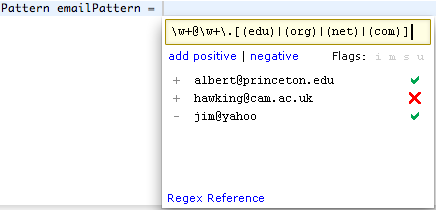
\includegraphics[width=\linewidth]{mockup-palette-small.png}
  \caption{An example mock-up palette for regular expressions shown to the survey participants. In the survey, they were shown the surrounding Eclipse IDE together.}
  \label{regex}
\end{figure}

Next, we presented participants with a series of mock-up palettes for a Color class, a regular expression class (Fig. \ref{regex}), and a SQL query class. Participants were also shown a mock-up demonstrating how a user could invoke the palette, and a mock-up showing the code that would be inserted once a selection had been made.

Before presenting each mock-up, we gathered information about the user's familiarity with the class and the strategies that they would likely use to instantiate the class under normal circumstances. For the Color class, the majority of participants indicated that they would look in the code completions menu (58.4\%) or in the class documentation (19.0\%) for a predefined constant. Another 14.0\% indicated that they would use an external tool to determine the RGB values. Few participants were unfamiliar with regular expressions and no participants were unfamiliar with SQL queries which provides further evidence that our participants were not novice developers. Fig. \ref{strategies} summarizes their usual strategies for instantiating regular expressions and SQL queries.

\begin{figure}
\begin{tabular}{lccc}
 & Regular Expressions &  & SQL\\
 \hline
Separate test script & 29.6\% &  & 15.4\%\\
Guess and check & 14.0\% &  & 16.1\%\\
External tool & \textbf{37.9\%} &  & \textbf{58.6\%}\\
Search for examples & 12.3\% & & 5.1\% \\
Other & 6.2\% & & 4.9\% \\
\hline
\end{tabular}
\caption{Typical strategies for regular expressions and SQL queries.}
\label{strategies}
\end{figure}


\begin{figure}
\begin{tabular}{crccccc}\\\\
\textsc{class}
& 
& \begin{rotate}{20}Nearly every time\end{rotate}
& \begin{rotate}{20}Most of the time\end{rotate}
& \begin{rotate}{20}Some of the time\end{rotate}
& \begin{rotate}{20}Rarely\end{rotate}
& \begin{turn}{20}Never\end{turn}\\
\hline
Color &\vline& 9.6\% & 22.1\% & \textbf{32.4\%} & 28.2\% & 7.7\%\\
RegExp &\vline& \textbf{36.6\%} & 29.5\% & 21.8\% & 7.3\% & 4.8\%\\
SQL & \vline &18.2\% & 19.3\% & \textbf{30.9\%} & 20.4\% & 11.4\%\\
\hline
\end{tabular}
\caption{The distribution of responses to the question: ``Consider situations where you need to instantiate the [specified] class. What portion of the time, in these situations, do you think you would use this feature?''}
\label{frequencies}
\end{figure}

Participants were positive about our mock-ups. We asked the users to rate the usefulness of each mock-up palette, and their responses are summarized in Fig. \ref{frequencies}. For each palette, more than half of the respondents expressed that they would use it at least some of the time. Especially, people liked the regular expression palette a lot.

\section{Design Implications}

We analyzed the open-ended responses to extract design principles and constraints. We got 193 responses for the color palette, 129 for the regular expression palette, and 142 for the SQL palette. Also, we got total 119 suggestions about what other types of classes could benefit from similar types of palettes. The extracted principles and constraints are summarized in the following subsections. The parenthesized number following each design constraint indicates how many people commented on that issue.

\subsection{System Design Constraints}

System design constraints are the criteria that should be taken into account in the design of the overall system architecture.

\subsubsection{Handling Separation of Concerns (183?)}

Participants were very wary of including constant data into the source code directly. Many responses expressed general sentiment or specific preference for project-wide color theme or external resource file. Sometimes they explicitly suggested to add capability to handle the external resource files directly from the palette. Interestingly, most people seemed to consider regular expressions as part of the program logic. There were few people who complained about including the regular expression pattern string in the source code as opposed to the other two classes.

%Examples of feedbacks in this category include:
%
%\begin{itemize}
%	\item The use of magic numbers in the source code is a bad design (54)
%	\item Color picking is the `designer's job' (33)
%	\item Would only use to define named constants (17)
%	\item Would rather use color scheme / theme (3)
%	\item Would use Object-Relational Mapping (ORM) / Language INtegrated Query (LINQ) instead of raw SQL query string (27 of 142)
%	\item These palettes might be useful for prototyping, but not for real production (14)
%	\item Instead of including the test cases into comments, they should be stored as unit tests (35 of 143)
%\end{itemize}
 
\subsubsection{Reversibility (19?)}

Some participants expressed that it should be able to bring the palettes back when they want to modify the parameters after they used the palettes.
 
\subsubsection{Palette Settings and State (41?)}

Many participants wanted to be able to configure the palettes or have the palettes maintain state even after the palettes are hidden. % The followings are the comments that are related to this category.

%\begin{itemize}
%	\item Want recently used regular expressions, and control over the comments (12)
%	\item Persistent database connection information is needed / want to manage connection pools (9)
%	\item Want recent colors, capability of setting favorite colors (20)
%\end{itemize}

\subsubsection{Interaction with Code Context (13?)}

Some people wanted to interact with the code context. For example, people expressed that it would be great if the SQL query palette was capable of dynamically creating SQL query string by combining multiple string variables, or by assigning variables for the parameters.

\subsubsection{Performance (?)}

Developers were concerned about the performance of these palettes. Some of the participants said that they would use these palettes only if it does not slow down the IDE. Also, this was the most popular comment on the reddit thread.

\subsubsection{IDE Independence (?)}

Several participants expressed a desire for IDE or even language independence for these palettes.

\subsection{General Palette Design Considerations}

General palette design considerations are about how to make more usable palettes.

\subsubsection{Simplicity vs. Capability}

Even though the participants were shown the same mockup screenshots, their reactions were split. Our color palette was considered too complex by many participants (26), and many others (26) would be satisfied with seeing colors next to a list of color names. The regular expressoin palette and SQL palette were considered too simple (12, and 15 participants respectively). They wanted syntax highlighting, match highlighting, and browsing capability of SQL databases.

\subsubsection{Keyboard Navigability (12)}

12 of the participants expressed strong antipathy toward the mouse. This was mostly directed at the color palette.

\subsection{Suggestions from the Participants}
At the end of the survey, we solicited suggestions from the participants about what types of classes could benefit from the active code completion palettes. 119 participants suggested various types of classes and we classified the suggestions into several categories.

\subsubsection{Alternative/Tricky/Literal Syntax (16)}
These are the classes of which syntax is tricky, or complex. Even for a basic string class, people wanted to input multiline string or unicode string in more convenient way with automatic escaping. We address this issue in more detail in Section \#.
%
%\begin{itemize}
%	\item Example classes
%	
%	\begin{itemize}
%		\item String
%		\item Collections (e.g., dictionary)
%		\item Vector, Matrix
%		\item Embedded languages
%		\item URLs, Paths
%	\end{itemize}
%	
%	\item Expected features
%	
%	\begin{itemize}
%		\item Proper escaping
%		\item Syntax highlighting
%		\item Auto-completion
%	\end{itemize}
%\end{itemize}

\subsubsection{Unclear Parameter Implications (11)}
The classes in this category has some parameters in it, and it is not easy to predict the results of the parameter modifications. Instead of running the whole application to see the result, the palette can serve as a preview panel so that the developers may check the results directly. Also, the palette can be a control panel which facilitates modifying the parameters as in Juxtapose [?].

%\begin{itemize}
%	\item Example classes
%	
%	\begin{itemize}
%		\item Audio tweaks (modifying pitch, volume, etc.)
%		\item 3D transformation matrices
%		\item number / string / date formatting
%		\item message box / input box (e.g., \texttt{JOptionPane})
%	\end{itemize}
%\end{itemize}

\subsubsection{Query Languages (17)}
Similar to the regular expression and SQL palette we presented, the developers also wanted to check if the other types of query strings (e.g., XPath / XQuery) are correct or not by checking the results directly on the palette.

%\begin{itemize}
%	\item Example classes
%	
%	\begin{itemize}
%		\item Regular expression
%		\item SQL query
%		\item XPath / XQuery
%	\end{itemize}
%\end{itemize}

\subsubsection{Graphical Elements (27)}
The other popular category was graphical elements. We've already shown the color example, and the participants suggested many other graphical properties such as font, brush, shape and others. Also, people wanted to check or directly manipulate the GUI frames and layouts.

%\begin{itemize}
%	\item Example classes
%	
%	\begin{itemize}
%		\item Color, Shape, Brush, Font, etc.
%		\item JFrame, Layouts, any swing components
%	\end{itemize}
%\end{itemize}

\subsection{Complex Instantiation Procedures (5)}
Some of the participants pointed out that these palettes might be useful to create an object which requires complex instantiation code. For example, in order to read a text file in Java, the developer might want to use \texttt{BufferedReader} class. It is error prone to use this class because it requires try/catch block, and also one must close the file after reading it. By using a palette to choose a file or choose a variable which contains the file path, the developers could easily instantiate these objects. In the same way, it can alleviate the factory pattern usability problem \cite{ellis_factory_2007}. As long as the developers remember which class to use, they will not need to remember how to instantiate that class.

%\begin{verbatim}
%BufferedReader reader = null;
%try {
%    reader = new BufferedReader(
%        new FileReader(filePath));
%} catch (IOException e) {
%    e.printStackTrace();
%}
%// use reader here
%reader.close();
%\end{verbatim}

\subsection{Describe by Example (2)}
Sometimes, it is possible to describe an object by examples. For instance, if there is a class which represents a shortcut key combination, we can easily instantiate an object of that class by pressing the actual shortcut key on the interactive palette.

%\begin{itemize}
%	\item Example classes
%	
%	\begin{itemize}
%		\item Keyboard Keys
%		\item Regular expression
%	\end{itemize}
%\end{itemize}

\subsection{Integrating with Documentation, Tutorial (7)}
Some participants suggested integrating the documentation or the tutorials into the interactive palettes. If the developers are not familiar of the specific API class, the palette could tell them how to use it.

% conference papers do not normally have an appendix


% use section* for acknowledgement
%\section*{Acknowledgment}


%The authors would like to thank...





% trigger a \newpage just before the given reference
% number - used to balance the columns on the last page
% adjust value as needed - may need to be readjusted if
% the document is modified later
%\IEEEtriggeratref{8}
% The "triggered" command can be changed if desired:
%\IEEEtriggercmd{\enlargethispage{-5in}}

% references section

% can use a bibliography generated by BibTeX as a .bbl file
% BibTeX documentation can be easily obtained at:
% http://www.ctan.org/tex-archive/biblio/bibtex/contrib/doc/
% The IEEEtran BibTeX style support page is at:
% http://www.michaelshell.org/tex/ieeetran/bibtex/
\bibliographystyle{IEEEtran}
% argument is your BibTeX string definitions and bibliography database(s)
\bibliography{vlhcc11}




% that's all folks
\end{document}


